
% ==========================
% main.tex — Scientific paper template
% Features:
%  • BibTeX (natbib) with a self-contained references.bib via filecontents*
%  • TikZ neural network diagram example
%  • Tables (booktabs + siunitx), figures, math (amsmath), theorems
%  • Code listings (listings; optional minted)
%  • PGFPlots example figure
%  • Clever cross-references + hyperlinks
% ==========================


\documentclass[11pt,a4paper]{article}

% --- Encoding, fonts, microtypography
\usepackage[T1]{fontenc}
\usepackage[utf8]{inputenc}
\usepackage{lmodern}
\usepackage{microtype}

% --- Page geometry
\usepackage[a4paper,margin=1in]{geometry}

% --- Math and theorem environments
\usepackage{amsmath,amssymb,amsfonts,mathtools}
\usepackage{amsthm}
\numberwithin{equation}{section}
\newtheorem{theorem}{Theorem}
\newtheorem{definition}{Definition}
\newtheorem{proposition}{Proposition}

% --- Figures, subfigures, graphics
\usepackage{graphicx}
\usepackage{subcaption}
\usepackage{float}

% --- Tables
\usepackage{booktabs}
\usepackage{multirow}
\usepackage{array}
\usepackage{siunitx}
\sisetup{detect-all=true, round-mode=places, round-precision=3}
\newcolumntype{C}[1]{>{\centering\arraybackslash}p{#1}}

% --- Code listings (simple, portable). For minted, see below.
\usepackage{listings}
\lstset{basicstyle=\ttfamily\small,columns=fullflexible,breaklines=true,frame=single,numbers=left,numberstyle=\tiny}
% Optional: \usepackage{minted} (requires -shell-escape and Pygments)

% --- Hyperlinks + Clever references
\usepackage{hyperref}
\hypersetup{colorlinks=true,linkcolor=blue,citecolor=blue,urlcolor=blue}
\usepackage[nameinlink,noabbrev]{cleveref}

% --- Bibliography (BibTeX via natbib)
\usepackage[numbers,sort&compress]{natbib}
\bibliographystyle{unsrtnat}

% --- Algorithms (choose one of these families)
% \usepackage{algorithm}
% \usepackage{algpseudocode}
% OR this convenient single-package alternative:
\usepackage[ruled,vlined]{algorithm2e}

% --- TikZ + PGFPlots for neural network diagrams and plots
\usepackage{tikz}
\usetikzlibrary{arrows.meta,positioning,calc,fit}
\usepackage{pgfplots}
\pgfplotsset{compat=1.18}

% Styles for NN drawings
\tikzset{
  neuron/.style={circle,draw,minimum size=15pt,inner sep=0,outer sep=0},
  input neuron/.style={neuron,fill=gray!10},
  hidden neuron/.style={neuron,fill=gray!20},
  output neuron/.style={neuron,fill=gray!10},
  connect/.style={-Latex}
}

% --- Title metadata
\title{Your Awesome Title: A Concise Scientific Paper Template}
\author{First Author$^{1}$ \and Second Author$^{2}$ \\
  \small $^{1}$Affiliation One \\ \small $^{2}$Affiliation Two}
\date{\today}

% --- Convenience macros (edit or remove as needed)
\newcommand{\R}{\mathbb{R}}
\newcommand{\E}{\mathbb{E}}
\newcommand{\Var}{\mathrm{Var}}

\begin{document}
\maketitle

\begin{abstract}
We present a minimal, modern \LaTeX{} template for scientific papers: Bib\TeX{} with \texttt{natbib}, neural network diagrams via TikZ, math and theorems, tables with \texttt{booktabs}/\texttt{siunitx}, code listings, and PGFPlots figures.\footnote{Repository-ready: drop in your own \texttt{references.bib} or keep the auto-generated one.}
\end{abstract}

\section{Introduction}
Cite seminal work with author-year commands, e.g., \citet{lecun2015deep} and grouped numeric-style citations \citep{kingma2014adam,he2016deep}. See \cref{sec:methods} for methods and \cref{sec:results} for results.

\subsection{Contributions}
\begin{itemize}
  \item A complete paper skeleton with sensible defaults.
  \item An inline TikZ example for a feed-forward neural network diagram (\cref{fig:nn}).
  \item Ready-to-use table and figure examples (\cref{tab:results,fig:plot}).
\end{itemize}

\section{Background}


The purpose of this paper is not only to showcase a surrogate model for all densities in the $\Lambda$CDM model but also to shine a light on the role of machine learning in Computational Physics. For that reason, in the background section we review both the physics and computational challenges of deriving the angular power spectrum, as well as the mathematical principles underlying neural networks, with particular emphasis on backpropagation. 

In what follows, we begin with a review of the physical origin and relevance of the angular power spectrum, followed by an overview of the tools used to simulate it. These being Bolztmann solvers such as CAMB and CLASS. 
We then proceed by motivating surrogate models and their usefulness in cosmology before diving in the mathematics of neural networks and their training via gradient descent. 
Finally, we outline the role of principal component analysis as a tool for dimensionality reduction in the context of building a surrogate to emulate the CMB power spectrum.


\subsection{Angular Power Spectrum}
\label{sec:aps}

\subsubsection{Physical origin of the CMB}

The CMB is the earliest possible electromagnetic image that we can currently observe. 
Prior to its release, the universe was a hot, dense plasma in which all components of the standard model were in thermal equilibrium with each other, including matter and radiation.  

In this tightly coupled state, photons interacted continuously with the surrounding plasma, primarily through Thomson scattering off free electrons
As a result, radiation could not propagate freely which made direct observation impossible.

To model the expanding universe during this epoch we use the \textbf{flat Friedmann–Lemaître–Robertson–Walker (FLRW) metric}

\begin{equation}
ds^2 = -c^2dt^2 + a^2(t)\left[dr^2 + r^2(d\theta^2 + \sin^2\theta d\phi^2) \right],
\end{equation}
Where $a(t)$ is the \textbf{scale factor} driving the expansion of the universe. 

As $a(t)$ grows the universe cools according to $T \propto 1/a(t)$. This cooling not only suppresses the average energy of photons, but also enables the formation of stable neutral hydrogen atoms. As a result, processes such as Thomson scattering ceased to be efficient, allowing photons to decouple from matter. These photons have since propagated freely across the universe, forming the Cosmic Microwave Background.
\subsubsection{Angular Power Spectrum}
Observationally, measurements of the CMB reveal that while the observed photon spectrum follows a nearly perfect blackbody with constant average temperature, a detailed analysis using the Planck distribution reveals tiny anisotropies. 

We can define the CMB temperature anisotropies as a function on the celestial sphere: 
\begin{equation}
  \Theta(\hat n) = \frac{\Delta T(\hat n)}{T}
\end{equation}

where $\hat n$ denotes a direction on the sky. Since the sky is a two-sphere, we can express this function in spherical harmonics as:
\begin{equation}
  \Theta(\hat n) = \sum_{\ell=0}^{\infty} \sum_{m = -\ell}^\ell a_{\ell m}Y_{\ell m}(\hat n).
\end{equation}

Because the CMB is well described as a nearly Gaussian random field, all of its statistical information is contained in its \textbf{two-point correlation} function:
\begin{equation}
  C(\theta) = \langle\Delta T(\hat n)\Delta T(\hat n')\rangle.
\end{equation}

Statistical isotropy then leads to: 
\begin{equation}
  \langle a_{\ell m} a_{\ell' m'}^*\rangle = C_{\ell} \delta_{\ell \ell'} \delta_{mm'}.
\end{equation}

Therefore the set of coefficients driving the spherical harmonic decomposition of $\Theta(\hat n)$ is completely described by the set of coefficients $\{C_\ell\}$, which make up the \textbf{angular power spectrum}. 

Currently our most precise measurement of the angular power spectrum was carried out by Planck 2018. Any viable cosmological theory must be able to reproduce the main features of that spectrum within uncertainty.  

% FIGURE placeholder: Planck 2018 angular power spectrum

Planck finds that the six-parameter $\Lambda$CDM model provides an excellent fit to the angular power spectrum. $\Lambda$CDM is characterized by the fractional energy densities of the main components of the Universe—baryons ($b$), dark matter ($\text{cdm}$), photons ($\gamma$), relativistic neutrinos ($\text{ur}$), dark energy ($\Lambda$), and curvature ($k$)—denoted by $\Omega_i$. These follow the Friedmann constraint:
\begin{equation}
\Omega_{\Lambda} + \Omega_k + \Omega_\text{cdm} + \Omega_b+ \Omega_\text{ur} + \Omega_\gamma = 1.
\end{equation}

While the Planck analysis is performed in terms of the following independent parameters $(\Omega_b h^2,\, \Omega_c h^2,\, 100\,\theta_s,\, \tau,\, n_s,\, \ln(10^{10}A_s))$,
these uniquely determine the values of the density fractions above. Varying these $\Omega_i$ allows us to study how each component of the cosmic fabric affects the CMB power spectrum. 

\subsection{Boltzmann Solvers}
\label{sec:boltzmann}

As mentioned above, Planck 2018 provides precise constraints that any cosmology should follow. To connect these observations with theory we must carry out a perturbed general relativistic treatment of how fluctuations in the early universe evolve with its expansion. As emphasized by Weinberg~\cite{weinberg2008}, the observed anisotropies in the CMB arise from several key physical effects:

\begin{itemize}
    \item Intrinsic temperature fluctuations in the photon–baryon plasma at last scattering ($z \simeq 1090$).
    \item Doppler effect from velocity perturbations of the plasma at recombination.
    \item Sachs–Wolfe effect: gravitational redshift or blueshift due to potential fluctuations at last scattering.
    \item Integrated Sachs–Wolfe effect: additional redshifts or blueshifts caused by time-varying gravitational potentials along the photon’s path from last scattering to today.
\end{itemize}

After a full treatment of these effects we arrive at the Einstein–Boltzmann equations, which must be solved for all species (photons, baryons, dark matter, neutrinos, dark energy) in order to accurately predict the CMB angular power spectrum. From linear theory we have that $C_\ell^{XY}$ ($X,Y \in \{T,E,B\}$) are given by:

\begin{equation}
C_\ell^{XY} = 4\pi \int_0^\infty \frac{dk}{k}\,
\mathcal{P}_{\mathcal{R}}(k)\, \Delta_\ell^X(k)\, \Delta_\ell^Y(k),
\end{equation}

where $\mathcal{P}_{\mathcal{R}}(k)$ is the primordial curvature power spectrum and 
$\Delta_\ell^X(k)$ are radiation transfer functions. These transfer functions are computed through the line-of-sight integral~\cite{seljak1996}:

\begin{equation}
\Delta_\ell^X(k) = \int_0^{\eta_0} d\eta \;
S_X(k,\eta)\, j_\ell\!\big(k[\eta_0-\eta]\big),
\end{equation}

with $j_\ell$ spherical Bessel functions and $S_X(k,\eta)$ the source functions encoding Sachs–Wolfe, Doppler, polarization, integrated Sachs–Wolfe, reionization, and lensing effects. 

% FIGURE placeholder: schematic of Einstein–Boltzmann hierarchy

Computing these source functions requires solving the full Einstein–Boltzmann hierarchy. For photons this takes the form

\begin{equation}
\dot\Theta_\ell = \frac{k}{2\ell+1}\big[\ell\,\Theta_{\ell-1} - (\ell+1)\,\Theta_{\ell+1}\big]
- \dot\tau\left(\Theta_\ell - \delta_{\ell 0}\Theta_0^{(\text{src})} - \delta_{\ell 1} v_b - \cdots\right),
\end{equation}

with $\dot\tau$ the Thomson scattering rate and $v_b$ the baryon velocity, coupled in turn to baryons, CDM, neutrinos, and metric perturbations. 

From the sctrcture of (2.9) alone we can already observe that computing the CMB power spectrum can be computationally expensive: each multipole $\Theta_\ell$ is coupled to its neighbors $\Theta_{\ell-1}$ and $\Theta_{\ell+1}$, producing a large system of coupled differential equations. To obtain accurate predictions up to small angular scales, the hierarchy must be evolved up to $\ell \sim 3000$, corresponding to thousands of coupled equations that must be solved for every Fourier mode $k$. 

To tackle this challenge, efficient \textbf{Boltzmann solvers} have been developed. Most notably these include \texttt{CAMB}~\cite{lewis2000} and \texttt{CLASS}~\cite{lesgourgues2011}. 
However, although these solvers are highly efficient and provide accurate theoretical predictions for comparison with Planck, the scale of the computation still means that each run can take seconds. 
While this compute time is fast enough for many applications, it is not suitable for fast \textbf{real-time applications}, thus motivating the creation of a \textbf{surrogate model}. 


\subsection{Surrogate Models}
\label{sec:surrogates}

As the fields of Data Analysis and Machine Learning evolve their impact extends across all areas of science, cosmology is being no exception. A prominent example of this influence is the adoption \textit{surrogate models}.

In this project, we focus on the use of neural networks (NN) as effective surrogates for predicting the temperature power spectrum of the CMB. 
However, much of the existing literature employing such techniques assumes that the reader is already familiar with their underlying principles. 
As a result, neural networks are often presented as opaque ‘black boxes,’ which can leave many researchers either unconvinced by their reliability or uninspired to engage with their use. In the next few sections of this paper we focus on building up these principles and answering why they make highly effective surrogates. 

\subsubsection{The Mathematics Behind Neural Networks}

A neural network can be thought of as a parameterized function $$f_\theta : A \to B$$ 
where $A$ denotes the space of inputs, $B$ the space of outputs, and $\theta$ the collection of learnable parameters. 
The idea is that neural networks approximate complex, often nonlinear, mappings by composing simple transformations.

$$
\text{(Two-step)}\quad
z_j = w_j h_{j-1} + b_j,\qquad h_j = \sigma_j(z_j),
$$
or equivalently

$$
\text{(One-line)}\quad
h_j = \sigma_j\!\big(w_j h_{j-1} + b_j\big),\qquad h_0 = x,
$$
with $w_j,b_j\in\mathbb{R}$. The network output is $f_\theta(x):=h_L$. In composed form, 

$$
f_\theta(x)=\sigma_L\!\Big(w_L\,\sigma_{L-1}\big(\cdots\,\sigma_1(w_1 x + b_1)\,\cdots\big)+b_L\Big).
$$
The parameters $\theta=\{(w_j,b_j)\}_{j=1}^L$ are initialized (typically randomly) and then trained on a dataset

$$
\mathcal{D}=\{(x^{(i)},y^{(i)})\}_{i=1}^N \subset \mathbb{R}\times\mathbb{R},
$$  
Where, $x^{(i)}$ denotes the $i$-th input sample, while $y^{(i)}$ is its corresponding output according to the mapping we aim to approximate. Thus the collection $\{x^{(i)}\}_{i=1}^N$ forms the set of inputs, and $\{y^{(i)}\}_{i=1}^N$forms the set of outputs otherwise known as \textbf{labels}.  

Now let $\mathcal{L}: \mathbb{R} \times \mathbb{R} \to [0, \infty)$ be an arbitrary \textbf{loss function} which measures the discrepancy between a predicted output $\hat y=f_\theta(x)$ and the true output $y$ (for example $\mathcal{L}(\hat y,y)=\tfrac12(\hat y-y)^2$). The average discrepancy over the training set is called \textbf{empirical risk}.

$$
J(\theta) \;=\; \frac{1}{N}\sum_{i=1}^N \mathcal{L}\!\big(f_\theta(x^{(i)}),\,y^{(i)}\big),
  \qquad \theta=\{(w_j,b_j)\}_{j=1}^L
$$
The objective during training is to find parameters that minimize $J(\theta)$. To find such set of parameters the network undergoes the \textbf{gradient descent}. Note that the gradient of the empirical risk with respect to the parameters is defined as: 


$$
\begin{aligned}
  w_j &\;\rightarrow\; w_j - \eta\,\frac{\partial J}{\partial w_j}, \quad j=1, \dots,L, 
  \\
  b_j &\;\rightarrow\; b_j - \eta\,\frac{\partial J}{\partial b_j}, \quad j=1, \dots,L,
  \\
\end{aligned}
$$

In practice we compute $\nabla_\theta J$ via \textbf{backpropagation}. Each step performs a forward pass to form predictions, computes the empirical risk against labels, backpropagates gradients, and updates parameters; an **epoch** is one full pass over the dataset, and training typically runs for multiple epochs.

The general case replaces scalars with vectors and matrices. For a layer of width $d_j$, let $h_{j-1}\in\mathbb{R}^{d_{j-1}}$, $W_j\in\mathbb{R}^{d_j\times d_{j-1}}$, and $b_j\in\mathbb{R}^{d_j}$. The forward map is

\begin{equation}
  h_j = \sigma_j\!\left(W_j h_{j-1} + b_j\right), 
  \qquad j = 1, \dots , L ,
\end{equation}
where $\sigma_j$ acts elementwise, and training, losses, and gradien-based optimization proceed exactly as in the scalar case.

The true potential of neural networks as surrogates directly stems from this formulation: once trained, the neural network is capable of reproducing our desired mapping using element wise nonlinearactivations and basic matrix multiplication.
Since these operations are highly optimized on modern hardware, evaluation using a NN compared to running full Bolztmann solvers becomes orders of magnitude faster. In theory, allowing for real-time predictions of the CMB power spectrum.

\subsubsection{}
\section{methodology}
\label{sec:methods}


\subsection{Neural network diagram (TikZ)}
\begin{figure}[H]
  \centering
  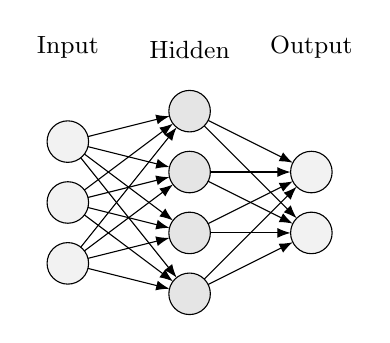
\begin{tikzpicture}[x=2.2em,y=2.2em]
    % Nodes: 3 inputs, 4 hidden, 2 outputs
    \foreach \i in {1,...,3} \node[input neuron]  (I\i) at (0,-\i) {};
    \foreach \i in {1,...,4} \node[hidden neuron] (H\i) at (2,-\i+0.5) {};
    \foreach \i in {1,...,2} \node[output neuron] (O\i) at (4,-\i-0.5) {};
    % Connections
    \foreach \i in {1,...,3} \foreach \j in {1,...,4} \draw[connect] (I\i) -- (H\j);
    \foreach \i in {1,...,4} \foreach \j in {1,...,2} \draw[connect] (H\i) -- (O\j);
    % Labels
    \node[above] at (0,0.2) {\small Input};
    \node[above] at (2,0.2) {\small Hidden};
    \node[above] at (4,0.2) {\small Output};
  \end{tikzpicture}
  \caption{Feed-forward neural network diagram drawn with TikZ.}
  \label{fig:nn}
\end{figure}

% Tip: For more complex diagrams, define macros or consider dedicated TikZ packages; this simple example avoids extra dependencies.

\subsection{Algorithm (pseudo-code)}
\begin{algorithm}[H]
\DontPrintSemicolon
\KwIn{Dataset $\{(x^{(i)},y^{(i)})\}_{i=1}^N$, learning rate $\eta>0$}
\KwOut{Trained parameters $\theta$}
Initialize $\theta$ randomly\;
\For{$t=1$ \KwTo $T$}{
  Sample mini-batch $\mathcal{B}$\;
  $g \leftarrow \nabla_{\theta} \frac{1}{|\mathcal{B}|}\sum_{(x,y)\in\mathcal{B}} \lVert f_{\theta}(x)-y\rVert^2$\;
  $\theta \leftarrow \theta - \eta\, g$\;
}
\caption{Mini-batch gradient descent}
\end{algorithm}

\subsection{A figure with PGFPlots}
\begin{figure}[H]
  \centering
  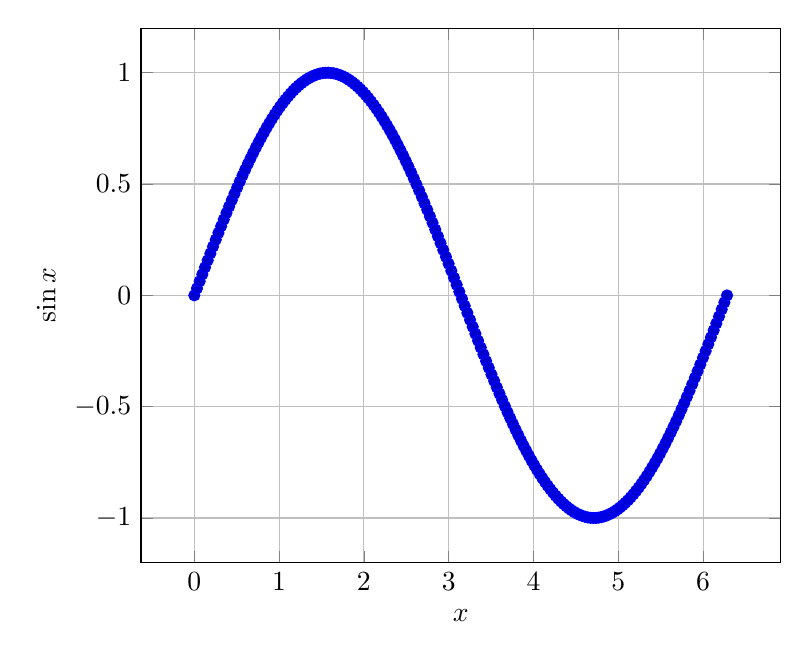
\begin{tikzpicture}
    \begin{axis}[
      width=0.8\linewidth,
      xlabel={$x$}, ylabel={$\sin x$},
      grid=both
    ]
      \addplot+[domain=0:6.283, samples=200] {sin(deg(x))};
    \end{axis}
  \end{tikzpicture}
  \caption{An example plot made with PGFPlots.}
  \label{fig:plot}
\end{figure}

\section{Results}
\label{sec:results}

\subsection{Tables}
Use \texttt{booktabs} for clean tables. \texttt{siunitx} aligns numbers by decimal separator.
\begin{table}[H]
  \centering
  \caption{Example results table.}
  \label{tab:results}
  \begin{tabular}{l S[table-format=1.3] S[table-format=1.3]}
    \toprule
    {Model} & {MSE $\downarrow$} & {Accuracy (\%)} \\
    \midrule
    Baseline  & 0.145 & 78.2 \\
    ResNet    & 0.092 & 84.5 \\
    Ours      & 0.054 & 88.7 \\
    \bottomrule
  \end{tabular}
\end{table}

\subsection{Code listing}
\begin{lstlisting}[language=Python,caption={PyTorch-style training step.}]
# Pseudocode
optimizer.zero_grad()
preds = model(x)
loss = torch.nn.functional.mse_loss(preds, y)
loss.backward()
optimizer.step()
\end{lstlisting}

\section{Discussion}
Discuss implications. For cosmology, see e.g. \citep{planck2018parameters,camb}.

\section{Conclusion}
Summarize contributions and future work.

\paragraph{Reproducibility Checklist}
Version your code/data, fix random seeds, log dependencies, and provide training details.

\section*{Acknowledgments}
Thank funding sources and collaborators here.

% --- References
% If you prefer biblatex + biber, switch packages; here we use BibTeX via natbib.
\bibliography{references}

\appendix
\section{Additional Material}
Extra proofs, ablations, or extended background.

% ==========================
% Build Tips
% ==========================
% FASTEST PATH (BibTeX):
%   pdflatex main
%   bibtex   main
%   pdflatex main
%   pdflatex main
%
% ONE-COMMAND (latexmk, auto-runs bibtex):
%   latexmk -pdf main.tex
%
% If you uncomment \usepackage{minted}, compile with:
%   pdflatex -shell-escape main
%   bibtex   main
%   pdflatex -shell-escape main
%   pdflatex -shell-escape main

\end{document}